%-------------------------------------------------------------------------------
% seq64_event_editor
%-------------------------------------------------------------------------------
%
% \file        seq64_event_editor.tex
% \library     Documents
% \author      Chris Ahlstrom
% \date        2016-01-02
% \update      2018-10-28
% \version     $Revision$
% \license     $XPC_GPL_LICENSE$
%
%-------------------------------------------------------------------------------

\section{Event Editor}
\label{sec:seq64_event_editor}

   The \textsl{Sequencer64 Event Editor} is used to view and edit,
   in detail, the events present in a sequence/pattern/track.
   This editor is not very sophisticated.
   It is a basic editor for simple edits and viewing.
   Viewing and scrolling generally work;
   editing, deleting, and inserting events work.
   But there are many possible interactions between event links (Note Off
   events linked to Note On events), performance triggers, and the pattern,
   performance, and event editor dialogs.
   Surely some bugs still lurk.
   If anything bad happens, do \textsl{not} press the
   \textbf{Save to Sequence} button!
   If the application aborts, let us know!

   Here are the major "issues":

   \begin{enumerate}
      \item It requires the user to know the details
         about MIDI events and data values.
      \item It does not present handy dropdown lists for various items.
      \item It does not detect any changes made to the sequence in the
         pattern editor, and so both editors cannot be brought on screen at the
         same time for the same pattern.
      \item It does not have an undo function.
      \item It cannot mark more than one event for deletion or modification.
      \item There is no support for dragging and dropping of events.
   \end{enumerate}

%  If, some day, we find ourselves needing
%  that kind of functionality, then we can add it.
%  There may also be issues with interactions between the event editor and
%  things like the performance editor and triggers.
   The event editor is a good way to see the events in a sequence,
   and to delete or modify problematic events.
   Additionally, it can be used to add \textbf{Set Tempo} meta events.
   \index{sequence extension}
   \index{pattern extension}
   If an event is added that has a time-stamp beyond the current
   length of the sequence, then the length of the sequence is extended.
   Unlike the event pane in the pattern editor, the event-editor
   dialog shows all types of events at once.

\begin{figure}[H]
   \centering 
%  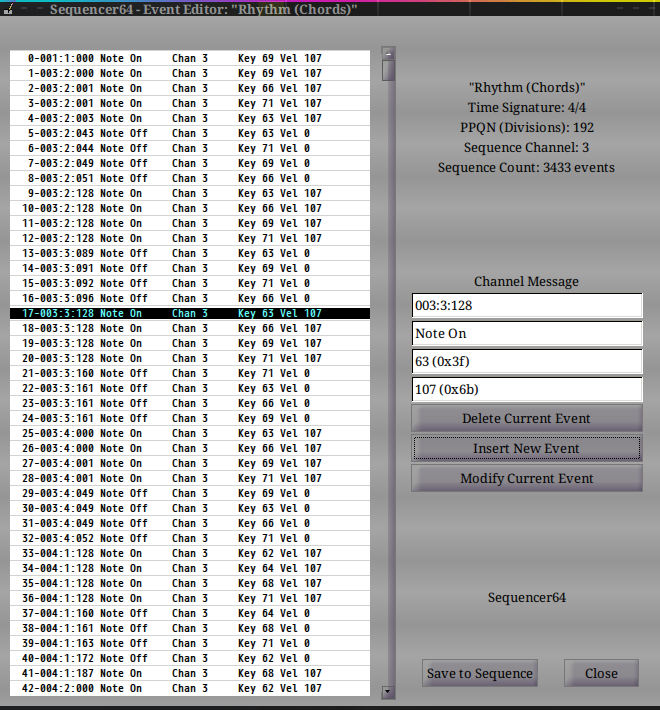
\includegraphics[scale=0.75]{event-editor/preliminary-event-editor.png}
   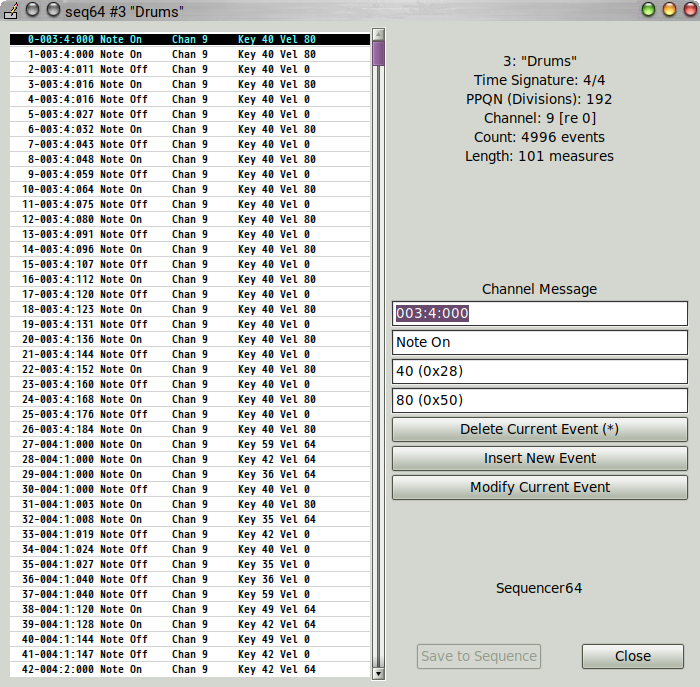
\includegraphics[scale=0.65]{new/event-editor-updated.png}
   \caption{Event Editor Window}
   \label{fig:event_editor_window}
\end{figure}

   The event-editor dialog is fairly complex.
   For exposition, we break it down into a few sections:

   \begin{enumber}
      \item \textbf{Event Frame}
      \item \textbf{Info Panel}
      \item \textbf{Edit Fields}
      \item \textbf{Bottom Buttons}
   \end{enumber}

   The event frame is a list of events, which can be traversed, and edited.
   The fields in the right panel show the name of
   the pattern containing the events and other information about the
   pattern.  The edit fields provide text fields for viewing and entering
   information about the current event, and buttons to delete, insert, and
   modify events.  The bottom buttons allow changes to be saved and the editor
   to be closed.  
   The following sections described these items in detail.

\subsection{Event Editor / Event Frame}
\label{subsec:seq64_event_editor_frame}

   The event frame is the event-list shown on the left side of the
   event editor.  It is accompanied by a vertical scroll-bar, for moving one
   line or one page at a time.
   Mouse or touchpad scrolling can be used to move up and down
   in the event list.  This movement is even easier than reaching for the
   scrollbars.

\subsubsection{Event Frame / Data Items}
\label{subsec:seq64_event_frame_data}

   The event frame shows a list of numbered events, one per line.
   The currently-selected event is highlighted in cyan text on a black
   background.  Here is an example of the data line for a MIDI event:

   \begin{verbatim}
      17-003:3:128 Note On   Chan 3    Key 66 Vel 107
   \end{verbatim}

   This line consists of the following parts:

   \begin{enumber}
      \item \textbf{Index Number}
      \item \textbf{Time Stamp}
      \item \textbf{Event Name}
      \item \textbf{Channel Number}
      \item \textbf{Data Bytes}
   \end{enumber}

   \setcounter{ItemCounter}{0}      % Reset the ItemCounter for this list.

   \itempar{Index Number}{event editor!index number}
   Displays the index number of the event.
   This number is purely for reference, and is not part
   of the event.  Events in the pattern are numbered from 0 to the number of
   events in the pattern.
%  They serve as a way to better know where one is in
%  the sequence.

   \itempar{Time Stamp}{event editor!time stamp}
   Displays the time stamp of the event,
   which indicates the cumulative time of the event in the pattern.
   It is displayed in the format of "measure:beat:divisions".
   The measure values start from 1, and range up to the number of measures in
   the pattern.
   The beat values start from 1, and range up to the number of beats in the
   measure.
   The division values range from 0 up to one less than the
   \index{ppqn}
   PPQN (pulses per quarter note) value for the whole song.
   \index{ppqn!\$ shortcut}
   As a shortcut, one can use the dollar sign ("\$") to represent
   PPQN-1.

   \itempar{Event Name}{event editor!event name}
   Displays the name of the event.
   The event name indicates what kind of MIDI event it is. 
   The following event names are supported:

   \begin{enumber}
      \item \textbf{Note Off}
      \item \textbf{Note On}
      \item \textbf{Aftertouch}
      \item \textbf{Control Change}
      \item \textbf{Program Change}
      \item \textbf{Channel Pressure}
      \item \textbf{Pitch Wheel}
      \item \textbf{Tempo}
   \end{enumber}

%  \textbf{Note that these are all MIDI \textsl{channel events}.
%  Support for MIDI \textsl{system events} is in place, but is not
%  ready for exposure to the user.}

   \itempar{Channel Number}{event editor!channel number}
   Shows the channel number (for channel-events only) re 0, not 1.
   For the user, of course, MIDI channels always range from
   1 to 16.  Internally, they range from 0 to 15.

   \itempar{Data Bytes}{event editor!data bytes}
   Shows the one or two data bytes for the event.

   Note Off, Note On, and Aftertouch events requires a byte for the key (0 to
   127) and a byte for the velocity (also 0 to 127).
   Control Change events require a control code and a value for that control
   code.  Pitch wheel events require two bytes to encode the full range of
   pitch changes.
   Program change events require only a byte value to pick the patch or program
   (instrument) to be used for the sequence.  The Channel Pressure event
   requires only a one-byte value.
   Tempo requires a number (e.g. "120.3") to be typed in.

\subsubsection{Event Frame / Navigation}
\label{subsec:seq64_event_frame_navigation}

   Moving about in the event frame is straightforward, but has some
   wrinkles to note.
%  (It was more difficult to get working than expected!)
   Navigation with the mouse is done by moving to the desired event and
   clicking on it.  The event becomes highlighted, and its data items are shown
   in the "info panel".
   There is no support for dragging and dropping events in the event frame.

   The scrollbar can be used to move within the frame, either by one line at a
   time, or by a page at a time.  A page is defined as one frame's worth of
   lines, minus 5 lines, for some overlap in paging.

   Navigation with keystrokes is also supported, for the Up and Down arrows and
   the Page-Up and Page-Down keys.  Note that using the Up and Down arrows by
   holding them down for awhile causes autorepeat to kick in, and the updates
   become very erratic and annoying.  Use the scrollbar or page keys to
   move through multiple pages.  Home and End also work.

\subsection{Event Editor / Info Panel}
\label{subsec:seq64_event_editor_info}

   The "info panel" is simply a read-only list of properties on the top right
   of the event editor.  It serves to remind the used of the pattern being
   edited and some characteristics of the pattern and the whole song.
   Five items are shown:

   \begin{enumber}
      \item \textbf{Sequence Number and Name}.
         A bit redundant, as the window caption for the event editor
         also shows the pattern name.
         It can be set in the pattern editor.
      \item \textbf{Time Signature}.
         A pattern property, shown only as a reminder.
         It can be set in the pattern editor.
      \item \textbf{PPQN}
         Shows the "parts per quarter note", or resolution of the
         whole song.  The default PPQN of \textsl{Sequencer64} is 192.
      \item \textbf{Sequence Channel}
         In \textsl{Sequencer64}, the channel number is a property of the
         pattern.  All channel events in the pattern get routed to the same
         channel, even if somehow the event itself specifies a different
         channel.
      \item \textbf{Sequence Count}
         Displays the current number of events in the pattern.
         This number changes as events are inserted or deleted.
   \end{enumber}

\subsection{Event Editor / Edit Fields}
\label{subsec:seq64_event_editor_fields}

   The edit fields show the values of the currently-selected event.  They allow
   changing an event, adding a new event, or deleting the currently-selected
   event.

   \begin{enumber}
      \item \textbf{Event Category} (read-only)
      \item \textbf{Event Timestamp}
      \item \textbf{Event Name}
      \item \textbf{Data Byte 1}
      \item \textbf{Data Byte 2}
      \item \textbf{Delete Current Event}
      \item \textbf{Insert New Event}
      \item \textbf{Modify Current Event}
   \end{enumber}

   \textbf{Important}: changes made in the event editor
   are \textsl{not} written to the sequence until the \textbf{Save to Sequence}
   button is clicked.  If one messes up an edit field, just click on the event
   again; all the fields will be filled in again.
   That's as much "undo" as the event-editor offers at this time, other than
   closing without saving.

   \setcounter{ItemCounter}{0}      % Reset the ItemCounter for this list.

   \itempar{Event Category}{event editor!event category}
   Displays the event category of the event.  Currently, only channel events
   can be handled, but someday we hope to handle the wide array of system
   events, and perhap even system-exclusive events.

   \itempar{Event Timestamp}{event editor!event timestamp}
   Displays the timestamp of the event.  Currently only the
   "measure:beat:division" format is fully supported.
   We allow editing (but not display) of the timestamp in
   pulse (divisions) format and "hour:minute:second.fraction" format, but
   there are bugs to work out.

   If one wants to delete or modify an event, this field does not need to be
   modified.  If this field is modified, and the \textbf{Modify Current Event}
   button is pressed, then the event will be moved.  This field can locate
   a new event at a specific time.  If the time is not in the current frame,
   the frame will move to the location of the new event and make it the current
   event.

   \itempar{Event Name}{event editor!event name}
   Displays the name of the event, and allows entry of an event name.
   The event name indicates what kind of MIDI event it is. 
   The following event names are supported:

   \begin{enumber}
      \item \textbf{Note Off}
      \item \textbf{Note On}
      \item \textbf{Aftertouch}
      \item \textbf{Control Change}
      \item \textbf{Program Change}
      \item \textbf{Channel Pressure}
      \item \textbf{Pitch Wheel}
      \item \textbf{Tempo}
   \end{enumber}

   Typing in one of these names changes the kind of event if the event is
   modified.  Abbreviations and case-insensitivity can be used to reduce the
   effort of typing.
   This handling of the editing of the event name is still a bit clumsy.
   It would be better to provide a drop-down list for more painless
   selection of events.  Some day.

   \itempar{Data Byte 1}{event editor!data byte 1}
   Allows modification of the first data byte of the event.
   One must know what one is doing.
   The scanning of the digits is very simple:  start with the first digit, and
   convert until a non-digit is encountered.  The data-byte value can be
   entered in decimal notation, or, if prepended with "0x", in hexadecimal
   notation.

   \itempar{Data Byte 2}{event editor!data byte 2}
   Allows modification of the second data byte of the event (if applicable
   to the event).
   One must know what one is doing.
   The scanning of the digits is as noted above.

   \itempar{Delete Current Event}{event editor!delete event}
   Causes the selected event to be deleted.
   The frame display is updated to move following events upward.

   \index{bugs!event delete key}
   \index{bugs!event insert key}
   \textsl{Sequencer64} would support using the Delete and Insert keys to
   supplement the buttons, but the Delete key is needed for editing the event
   data fields.
   The current structure of the dialog prevents using it for both
   the frame and the edit fields.  Therefore, \textsl{Sequencer64} allows the
   usage of the \textbf{asterisk} keys (regular and keypad) for
   deletion.

   \itempar{Insert New Event}{event editor!insert event}
   Inserts a new event, described by the 
   \textbf{Event Timestamp},
   \textbf{Event Name},
   \textbf{Data Byte 1}, and
   \textbf{Data Byte 2} fields.
   The new event is placed in the appropriate location for the given timestamp.
   If the timestamp is at a time that is not visible in the frame, the frame
   moves to show the new event, so be careful.

   \itempar{Modify Current Event}{event editor!modify event}
   Deletes the current event, and inserts the modified event,
   which is placed in the appropriate location for the given
   timestamp.

\subsection{Event Editor / Bottom Buttons}
\label{subsec:seq64_event_editor_buttons}

   The buttons at the bottom of the event editor round out the functionality of
   this dialog.

   \begin{enumber}
      \item \textbf{Save to Sequence}
      \item \textbf{Close}
   \end{enumber}

   \setcounter{ItemCounter}{0}      % Reset the ItemCounter for this list.

   \itempar{Save to sequence}{event editor!save to sequence}
   Saves the event container back to the sequence from
   whence the events came.  This button does not close the dialog; further
   editing can be performed.  The Save button is enabled only if
   some unsaved changes to the events exist.
%  Note that there may still be some subtle bugs in the dialog editor, so be
%  careful about pressing this button.

   Any sequence/pattern editor that is open should be reflected
   in the pattern editor once this button is pressed.  However, at present,
   simultaneous use of the pattern editor and event editor has been disabled.
   \index{bugs!event delete segfault}
   If both the event editor and the pattern editor are open for a sequence
   (currently disabled), and
   some events are deleted in the event editor, and the
   \textbf{Save to Sequence} button is pressed, the pattern editor would
   crash and
   takes down \textsl{Sequencer64} with it.  Therefore, when either editor is
   open for a given sequence, the right-click menu entries that bring them up
   are hidden.

   \itempar{Close}{event editor!close}
   Closes the event editor.
   Any unsaved event changes are discarded.
   There is a "modification indicator" to show that the events have
   been modified.

   Again, good luck with the dialog.  Bug reports are appreciated.

%-------------------------------------------------------------------------------
% vim: ts=3 sw=3 et ft=tex
%-------------------------------------------------------------------------------
